\documentclass[a4paper,10pt]{article}
\usepackage[utf8]{inputenc}
\usepackage{graphicx}

\title{BSIP: Separating uterine EMG records using sample entropy }
\author{Neža Belej (63120340)}

\begin{document}

\maketitle

\section {Introduction}
Uterine electromyogram (EMG), also termed electrohysterogram (EHG), represents electrical activity of uterus. The EHG signals contain also intervals with increased electrical activity of uterus. The increased electrical activity is visible in the EHG signals as short bursts with higher signal amplitude. These intervals usually coincide with contractions. (But not all intervals with increased electrical activity of the uterus are a result of contractions.) The frequency contents of the EHG signals changes during contractions, but the studies have also shown, that the frequency contents of the EHG signals as well as frequency contents of individual contractions within a signal, changes as the labour approaches.  Our task was to analyse 4 different records and their sample entropies: 

\begin{itemize}
\item{PE (pre-term labor, recorded before 26th week)}
\item{PL (pre-term labor, recorded during or after 26th week)}
\item{ TE (term labor, recorded before 26th week)}
\item{TL (term labor, recorded during or after 26th week)}
\end{itemize}

\section {Terms}

\begin{itemize}
\item{Sample entropy is a measure of regularity of finite length time series and estimates the extent to which the data did not arise from a random process. Less predictable time series exhibit a higher sample entropy. \\  When the labor is aproaching, the power spectrum is moving to lower frequencies which makes the signal more predictable. Therefore, the sample entropy is lower because of higher predictability.}
\item{The Butterworth filter is a type of signal processing filter designed to have as flat a frequency response as possible in the passband. It has a smooth frequency response
and is computationally non intensive.\\ Filter can be high-pass, low-pass or band-pass. \\
We used band-pass filter with bandpass between 0.3 - 4 Hz.}
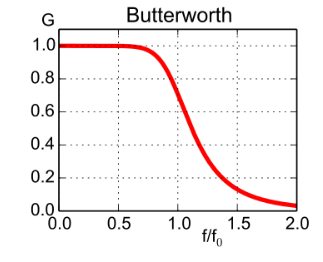
\includegraphics{butter}
\end{itemize}

\section {Results}

\begin{itemize}
\item{Sample entropy of PE (3.signal): 1.5805}
\item{Sample entropy of PE (2.signal): 1.0367}
\item{Sample entropy of PL (3.signal): 1.2150}
\item{Sample entropy of TE (3.signal): 1.9926}
\item{Sample entropy of TL (3.signal): 1.6447}
\end{itemize}

\section {Conclusion}
\begin{itemize}
\item{Sample entropy of PE is higher than sample entropy of PL, which was expected because when the labour is close, contractions are more regular and predictability of signal is higher. }
\item{Sample entropy of TE is higher than sample entropy of TL, which was expected because when the labour is close, contractions are more regular and predictability of signal is higher. Both values are also higher than results for PE and PL which was also expected.}
\item{Sample entropy of TE is higher than sample entropy of PE, which was expected because the predictability of pre-term record must be higher, because the power spectrum already moved to lower frequencies which corresponds to higher predictability and lower sample entropy values.}
\item{Sample entropy of TL is higher than sample entropy of PL, which was expected because the predictability of pre-term record must be higher, because the power spectrum already moved to lower frequencies which corresponds to higher predictability and lower sample entropy values.}
\item{For signal 2 we get lower value which means that the predictability of signal 2 is much higher than signal 3.}
\end{itemize}


\end{document}


